%%%%%%%%%%%%%%%%%%%%%%%%%%%%%%%%%%%%%%%%%%%%%%%%%%%%%%%%%%%%%%%%%%%%%%%%%%%%%%%%

\section{Řešení}
\label{sec_solution}

\subsection{Vytvoření trénovací sady}

Pomocí nástroje pro vývojáře mobilních aplikací Android Studio\footnote{\url{https://developer.android.com/studio}} byl vytvořen virtuální mobilní telefon Google Pixel 4XL s~operačním systémem Android 11 a procesorovou architekturou x86.

Jelikož na takto vytvořený virtuální telefon není možné instalovat aplikace přes vestavěný klient Google Play, bylo nutné využít repozitáře třetích stran ApkMirror\footnote{\url{https://apkmirror.com}} nebo ApkPure\footnote{\url{https://apkpure.com}} a aplikace nainstalovat manuálně. Byl nainstalován následující seznam aplikací:

\begin{enumerate}
    \item \textit{Yr} v5.13.2,
    \item \textit{Settle Up: Group Expenses} v10.0.2030,
    \item \textit{Forest: Stay focused} v4.35.1,
    \item \textit{Forza Football: Live soccer scores} v5.1.13,
    \item \textit{Revolut} v7.43.1,
    \item \textit{GitHub} v1.7.4,
    \item \textit{Netflix} v7.97.1,
    \item \textit{Twitter} v8.88.0,
    \item \textit{YouTube} v16.12.34,
    \item \textit{Phoenix: The Bitcoin wallet from the future} v1.4.8.
\end{enumerate}

\begin{figure}[H]
    \centering
    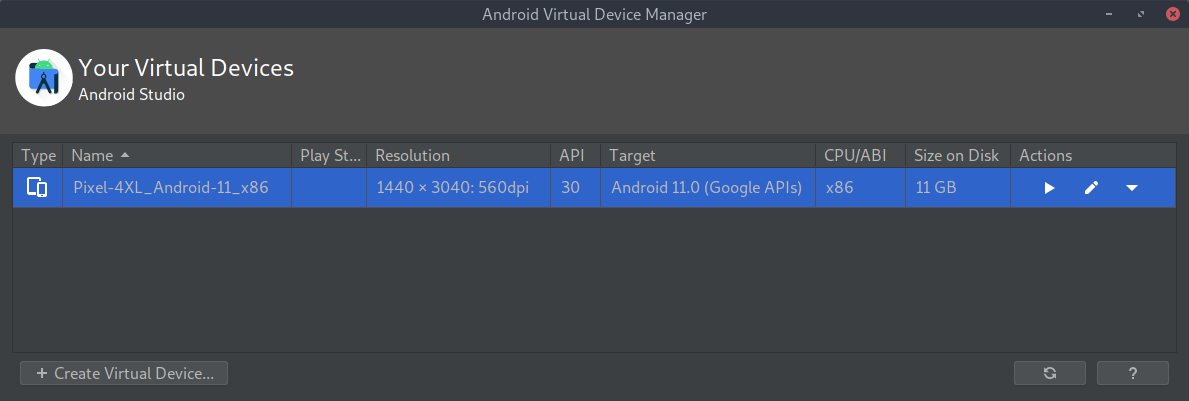
\includegraphics[width=0.99\linewidth]{android_virtual_device_manager.png}
    \caption{Program Android Virtual Device Manager pro správu virtuálních mobilních zařízení.}
    \label{fig_android_virtual_device_manager}
\end{figure}

\begin{center}
    \begin{lstlisting}[
        language=bash,
        caption={Spuštění virtuálního mobilního telefonu přes příkazový řádek na konkrétním portu.}
    ]
$ emulator -avd Pixel-4XL_Android-11_x86 -port 12345
\end{lstlisting}
\end{center}

\begin{figure}[H]
    \centering
    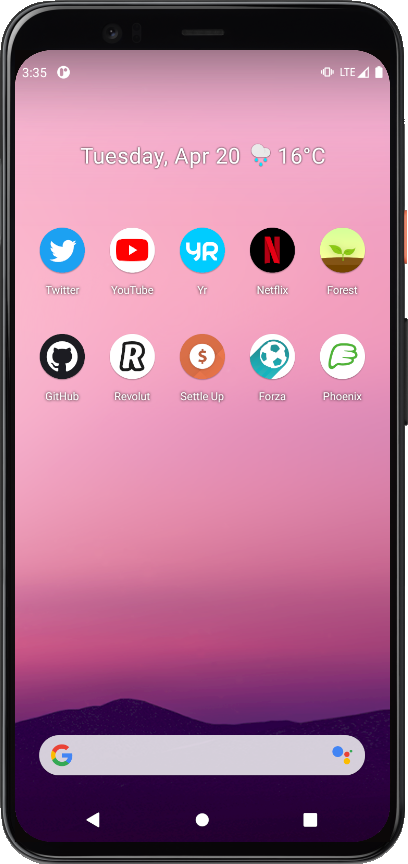
\includegraphics[width=0.25\linewidth]{google_pixel_4xl.png}
    \caption{Virtuální mobilní telefon Google Pixel 4XL s~operačním systémem Android 11 a nainstalovanými testovacími aplikacemi.}
    \label{fig_google_pixel_4xl}
\end{figure}

Pomocí klienta \texttt{adb} (\textit{Android Debug Bridge})\footnote{\url{https://developer.android.com/studio/command-line/adb}} je možné komunikovat s~virtuálním telefonem skrze příkazový řádek. Pro simulaci provozu jednotlivých aplikací byl použit nástroj \texttt{monkeyrunner}.\footnote{\url{https://developer.android.com/studio/test/monkeyrunner}} Ten lze přes \texttt{adb} spustit uvnitř telefonu. Programem Wireshark\footnote{\url{https://www.wireshark.org}} je možné poté odposlechnout síťový provoz a uložit jej jako \texttt{pcap} soubor.

\begin{center}
    \begin{lstlisting}[
    language=bash,
    caption={Spuštění 1000 náhodných událostí aplikace Phoenix.}
]
$ adb -s emulator-12345 shell monkey -p fr.acinq.phoenix.mainnet \ -v 1000
\end{lstlisting}
\end{center}

\begin{figure}[H]
    \centering
    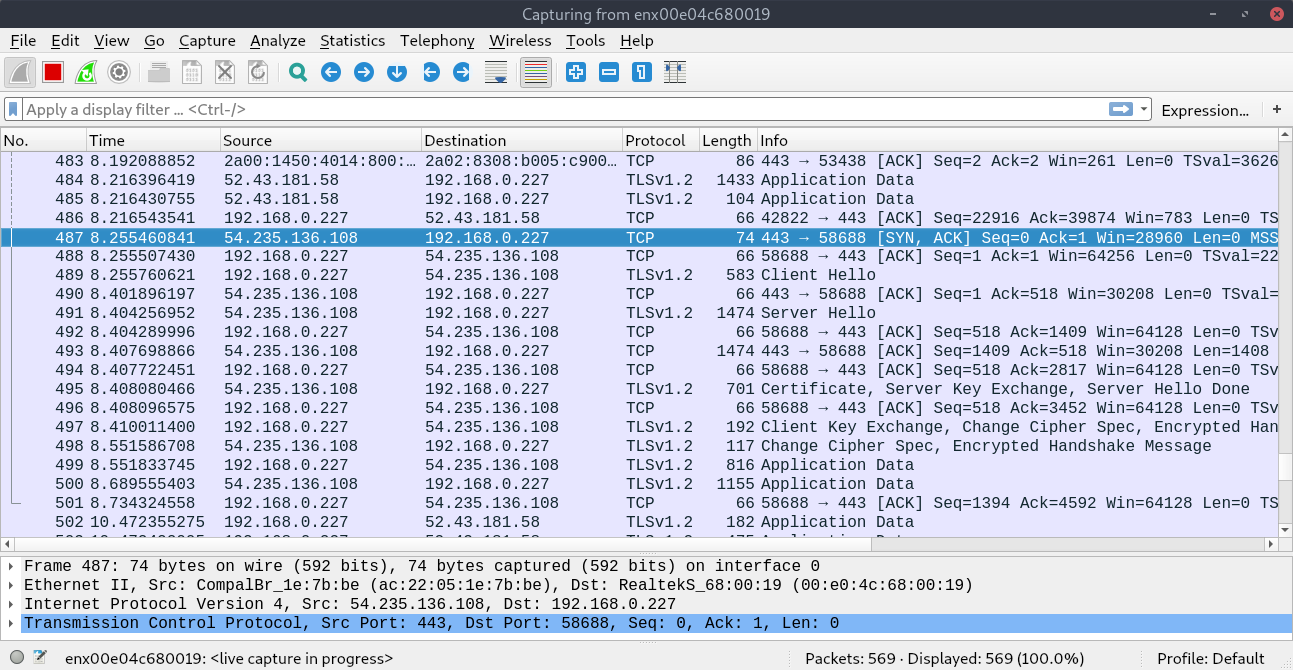
\includegraphics[width=0.99\linewidth]{wireshark.png}
    \caption{Zaznamenávání síťového provozu na virtuálním mobilním zařízení pomocí aplikace Wireshark.}
    \label{fig_wireshark}
\end{figure}

Tímto způsobem byla postupně zaznamenána komunikace každé z~vybraných aplikací. Celý postup byl opakován $6\times$. Celkově tedy bylo sesbíráno $60$ trénovacích \texttt{pcap} souborů. V~každém z~nich byla zaznamenána síťová komunikace během $1000$ náhodných událostí aplikace vyvolaných nástrojem \texttt{monkeyrunner}.

\subsection{Zpracování trénovací sady}

Pro zpracování \texttt{pcap} souborů byl využit jazyk Python a knihovna Pyshark\footnote{\url{https://github.com/KimiNewt/pyshark}}. Pyshark pouze zaobaluje Tshark\footnote{\url{https://www.wireshark.org/docs/man-pages/tshark.html}}, což je terminálová verze Wiresharku, do Python knihovny.

Zachycený provoz aplikací neobsahuje pouze komunikaci mezi telefonem a serverem aplikace samotné, ale také komunikace aplikací na pozadí a spojení s~reklamními a analytickými servery. Tyto spojení je nutné odfiltrovat. To bylo provedeno na základě sestavení \textit{whitelistu} podřetězců serverů (doménové jméno serveru musí obsahovat daný podřetězec), pro jednotlivé aplikace. Doménová jména serverů byla vypozorována z~komunikace jednotlivých aplikací.

\begin{center}
    \begin{lstlisting}[
        language=bash,
        caption={\textit{Whitelist} podřetězců komunikujících serverů pro jednotlivé aplikace.}
    ]
{
  "revolut": ["revolut"],
  "twitter": ["twitter", "twimg"],
  "phoenix": ["phoenix", "acinq"],
  "netflix": ["netflix", "nflxext"],
  "forza": ["forza"],
  "youtube": ["youtube", "ytimg", "redirector.googlevideo"],
  "yr": ["yr"],
  "forest": ["forest", "seekrtech"],
  "github": ["github"],
  "settleup": ["settleup", "settle-up"]
}
\end{lstlisting}
\end{center}

Z~veškeré zachycené komunikace byly vyfiltrovány TLS \textit{Client Hello} a TLS \textit{Server Hello} packety. Z~vybraných položek \textit{Handshake Version}, \textit{Cipher Suites}, \textit{Extensions}, \textit{Supported Groups} a \textit{Elliptic Curve Point Format} byl spočítán JA3 otisk pomocí hashovací funkce MD5. Takto byl spočítán otisk každého vyfiltrovaného packetu. Ze seznamů \textit{Cipher Suites}, \textit{Supported Groups} a \textit{Extensions} byly vymazány hodnoty GREASE (\textit{Generate Random Extensions And Sustain Extensibility}), \textit{renegotiation} a \textit{padding}. Které se objevují náhodně, případně jsou redundantní a do komunikace zavádějí nedeterminismus~\cite{bib_matousek}.

\begin{center}
    \begin{lstlisting}[
        language=bash,
        caption={Příklad výpočtu JA3 otisku z~TLS \textit{Client Hello} packetu.}
    ]
{
  "handshake_version": "771",
  "cipher_suites": "49195,49196,52393,49199,49200,52392,49171,49172,156,157,47,53",
  "extensions": "0,23,10,11,5,13",
  "supported_groups": "29,23,24"
  "ec_point_format": "0",
  "ja3_fingerprint": "2595ab65e691eb1d942c6094ff92c933"
}
\end{lstlisting}
\end{center}

Příznaky aplikací tvoří trojice následujícího formátu: JA3 otisk spočítáný z~TLS \textit{Client Hello}, JA3 otisk spočítaný z~TLS \textit{Server Hello} a SNI (\textit{Server Name Indication}), tedy doménové jménu serveru. Každé aplikaci připadá seznam příznaků. Všechny příznaky byly uloženy do souboru formátu \texttt{json}.

Odpovídající packety \textit{Client Hello} a \textit{Server Hello} byly propojeny na základě zdrojové/cílové IP adresy a zdrojového/cílového portu.

\begin{center}
    \begin{lstlisting}[
        language=bash,
        caption={Ukázka z~trénovací sady, příznaky aplikace Phoenix.}
    ]
{
  ...
  "phoenix": [
    {
      "client_ja3": "709c6b4bc7678a83ccc13a529103c873",
      "server_ja3": "77f87cbba1f72fcf7fbc308d9dcb561d",
      "sni": "phoenix.acinq.co"
    },
    {
      "client_ja3": "2595ab65e691eb1d942c6094ff92c933",
      "server_ja3": "b5c7a4c92e1f26c18a37bc9c1acd64b5",
      "sni": "acinq.co"
    },
    {
      "client_ja3": "cb533a60549e1e6021bd620b77ffce72",
      "server_ja3": "9758f7a0e1460a60e317ae2131b733a5",
      "sni": "electrum.acinq.co"
    }
  ],
  ...
}
\end{lstlisting}
\end{center}

%%%%%%%%%%%%%%%%%%%%%%%%%%%%%%%%%%%%%%%%%%%%%%%%%%%%%%%%%%%%%%%%%%%%%%%%%%%%%%%%
